% ============================================================
% Dissertation Proposal — Spot To Go
% Word Count: ~3000 words (excluding bibliography)
% ============================================================

\documentclass[12pt, a4paper]{article}

% --- Packages ---
\usepackage[margin=2.5cm]{geometry}
\usepackage{setspace}
\usepackage{titlesec}
\usepackage{parskip}
\usepackage{hyperref}
\usepackage{pgfgantt}
\usepackage{booktabs}
\usepackage{array}
\usepackage{natbib}
\usepackage{times}
\usepackage{graphicx}
\usepackage{float}
\usepackage{tikz}
\usetikzlibrary{arrows.meta}

\doublespacing

% --- Section formatting ---
\titleformat{\section}{\large\bfseries}{\thesection.}{0.5em}{}
\titleformat{\subsection}{\normalsize\bfseries}{\thesubsection}{0.5em}{}

% ============================================================
\begin{document}

% --- Title Block ---
\begin{center}
    {\LARGE \textbf{Spot To Go: A Location-Based Android Application}} \\[0.5em]
    {\large \textbf{for Restaurant Discovery with Video Integration}} \\[1.5em]
    {\normalsize Dissertation Proposal} \\[0.3em]
    {\normalsize Word Count: 3,000 words (excluding bibliography)} \\[2em]
\end{center}

\hrule
\vspace{2em}

% ============================================================
\section{Background and Description of the Proposed Project}

The rapid adoption of smartphones has changed the way people navigate their daily environments. Mobile applications have become a primary tool for decision-making — particularly in areas such as food discovery, navigation, and local exploration.

Existing platforms such as Google Maps, Yelp, and Zomato have established themselves as widely used tools in this space. They provide users with location-based search results, star ratings, and written reviews. While these features are functional and well-integrated, they share a common limitation: the information they provide is largely static and text-driven. A restaurant's atmosphere, food presentation, and overall dining experience are difficult to communicate through a numerical rating or a short written comment alone.

At the same time, platforms such as YouTube and TikTok have demonstrated that short-form video content is one of the most effective formats for communicating real-world experiences. Consumers increasingly rely on video reviews and walkthroughs before making decisions about restaurants, travel, and products. Research in consumer behavior confirms that visual and experiential content builds significantly stronger trust and engagement than text-based reviews \citep{dellarocas2003, cheung2009}. Despite this, no widely available tool currently combines map-based restaurant discovery with direct access to video content in a seamless mobile experience.

This project addresses that gap. ``Spot To Go'' is a proposed Android mobile application designed to allow users to discover nearby restaurants on an interactive map and access real-life video previews — sourced from YouTube or TikTok — associated with each restaurant. The application populates the map based on the user's GPS location; users can tap any restaurant to view its details and watch an associated video.

Beyond its functional purpose, this project serves as a structured learning exercise in Android application development, drawing on established technologies including the Google Maps SDK, the Google Places API, the Fused Location Provider, and Android's Activity-based architecture.

% ============================================================
\section{Aim and Objectives}

\subsection*{Aim}

The aim of this project is to design and develop an Android mobile application that enables users to discover nearby restaurants through an interactive, location-aware map interface and access associated video content to support informed decision-making.

\subsection*{Objectives}

The following objectives define the scope of the project and provide a measurable framework against which its success can be evaluated:

\begin{enumerate}
    \item To integrate the Google Maps SDK to render an interactive map centered on the user's real-time GPS location.

    \item To implement location-based restaurant discovery using the Google Places API, displaying nearby restaurants as interactive map markers.

    \item To develop a restaurant detail screen that presents structured information — including name, rating, distance, and description — in a clear and accessible format.

    \item To integrate video content from YouTube or TikTok by associating each restaurant with a corresponding video preview, accessible directly from within the application.

    \item To implement a navigation feature that launches Google Maps directions from the user's current location to a selected restaurant.

    \item To design and implement a keyword-based search interface that allows users to filter nearby restaurant results based on text input.

    \item To evaluate the application through functional testing against each objective, verifying that all core features operate correctly under standard usage conditions.
\end{enumerate}

These objectives are arranged in order of development priority and correspond to the phases outlined in the work plan.

% ============================================================
\section{Critical Review of Related Literature}

The development of ``Spot To Go'' is informed by four interconnected areas of research: location-based services, restaurant recommendation systems, the role of video-based user-generated content in consumer decision-making, and Android mobile application development.

\subsection{Location-Based Services}

Location-based services (LBS) refer to systems that use the geographic position of a device to deliver contextually relevant information or functionality to the user. \citet{schiller2004} provide a foundational framework for understanding LBS, describing how the combination of GPS positioning, mobile networks, and application logic enables a new class of context-sensitive applications.

\citet{dey2001} extends this through the notion of context-aware computing — systems that adapt to the user's physical environment rather than requiring manual configuration. In this project, the user's GPS position is read automatically, with no manual location input required.

More recent work by \citet{bao2012} demonstrates that combining location data with user preference modeling improves the relevance of place-based recommendations. This project does not implement such a model, though the architecture is designed to accommodate it in future.

\subsection{Restaurant Recommendation Systems}

The problem of identifying relevant restaurants for a given user has been approached through a range of algorithmic methods. \citet{adomavicius2005} offer a comprehensive review of recommender system techniques, identifying content-based filtering, collaborative filtering, and hybrid approaches as the dominant paradigms.

For this project, a simplified form of content-based filtering is adopted: keyword-based search against the Google Places API. This approach retrieves results based on the match between the user's search input and the restaurant's name or type. It is intentionally lightweight — appropriate given the academic scope of the project — while still demonstrating a functional and responsive discovery mechanism. The Google Places API itself incorporates community ratings and review counts, which represent a form of aggregated collaborative signal. This means the data source carries recommendation intelligence without requiring the application to implement it independently.

\subsection{Video-Based User-Generated Content and Consumer Decisions}

The influence of user-generated content on consumer behavior is a well-established area of study. \citet{dellarocas2003} identifies online reviews and community-generated content as a digital extension of word-of-mouth communication, arguing that such content exerts a measurable and statistically significant influence on purchasing decisions. \citet{kaplan2010} expand on this observation in the context of social media platforms, noting that video content has emerged as the dominant format for influencing consumer decisions — not merely because of its popularity, but because it communicates atmosphere, authenticity, and experiential quality in ways that text and static images fundamentally cannot.

\citet{cheung2009} specifically examine the impact of electronic word-of-mouth in the context of trust and decision confidence, finding that visual content generates significantly higher levels of credibility than text-based equivalents. This finding is directly relevant to restaurant selection, where factors such as food quality, ambiance, and service style are inherently visual and experiential. A written review may describe these qualities, but a short video demonstrates them.

\subsection{Android Mobile Application Development}

\citet{wasserman2010} identifies several challenges specific to mobile application development, including device fragmentation, limited processing resources, and the complexity of managing application state across screen rotations and background interruptions. The Android Activity lifecycle addresses the state management challenge by providing a structured, event-driven framework in which each screen is an independent, lifecycle-aware component. This architecture forms the structural backbone of the proposed application.

While Kotlin has become Google's preferred language for new Android development since 2017, Java remains fully supported and continues to be widely used in educational contexts due to its extensive documentation, longer track record, and closer alignment with prior object-oriented programming instruction. This project uses Java in accordance with the project brief, and the choice imposes no limitation on the APIs or features available within the Android ecosystem.

The Google Play Services suite — comprising the Maps SDK, the Places API, and the Fused Location Provider — provides a standardized set of tools that abstract the complexity of location-aware development on Android. These tools are maintained by Google and extensively documented, making them suitable for both academic and practical use.

% ============================================================
\section{Methodologies and Methods}

\subsection{Development Methodology}

The project follows an Agile development approach, organized into iterative phases. Each phase delivers a testable increment, allowing technical issues to be identified before the next phase begins. This approach is well-suited to a project where learning is an explicit objective alongside delivery.

\subsection{Development Environment and Tools}

The application is built using Android Studio, which provides an integrated development environment with built-in support for emulation, debugging, and layout design. Java is used as the primary programming language, in line with the project brief. The minimum supported Android SDK version is set to API level 24 (Android 7.0 Nougat), which ensures compatibility with the majority of active Android devices.

Version control is managed using Git, with commits structured around each development phase.

\subsection{Application Architecture}

The application follows a single-Activity-per-screen architecture, in which each screen is implemented as a discrete Android Activity. This structure is straightforward to implement and aligns with the separation-of-concerns principle. The screen hierarchy is as follows:

\begin{itemize}
    \item \textbf{LoginActivity / RegisterActivity} — Provides the login and registration screens to demonstrate the authentication workflow. These screens are not backed by a live service; access is granted using hardcoded sample credentials.
    \item \textbf{MainActivity} — Provides the home screen with a keyword search bar.
    \item \textbf{MapActivity} — Renders the interactive map and restaurant markers.
    \item \textbf{RestaurantDetailActivity} — Displays structured restaurant information and action buttons.
    \item \textbf{VideoActivity} — Presents the associated restaurant video via WebView or Intent.
    \item \textbf{DirectionsActivity} — Launches Google Maps navigation to the selected restaurant.
\end{itemize}

Each Activity is responsible for one clearly defined task, and data is passed between screens using Android's Intent mechanism.

\begin{figure}[h!]
    \centering
    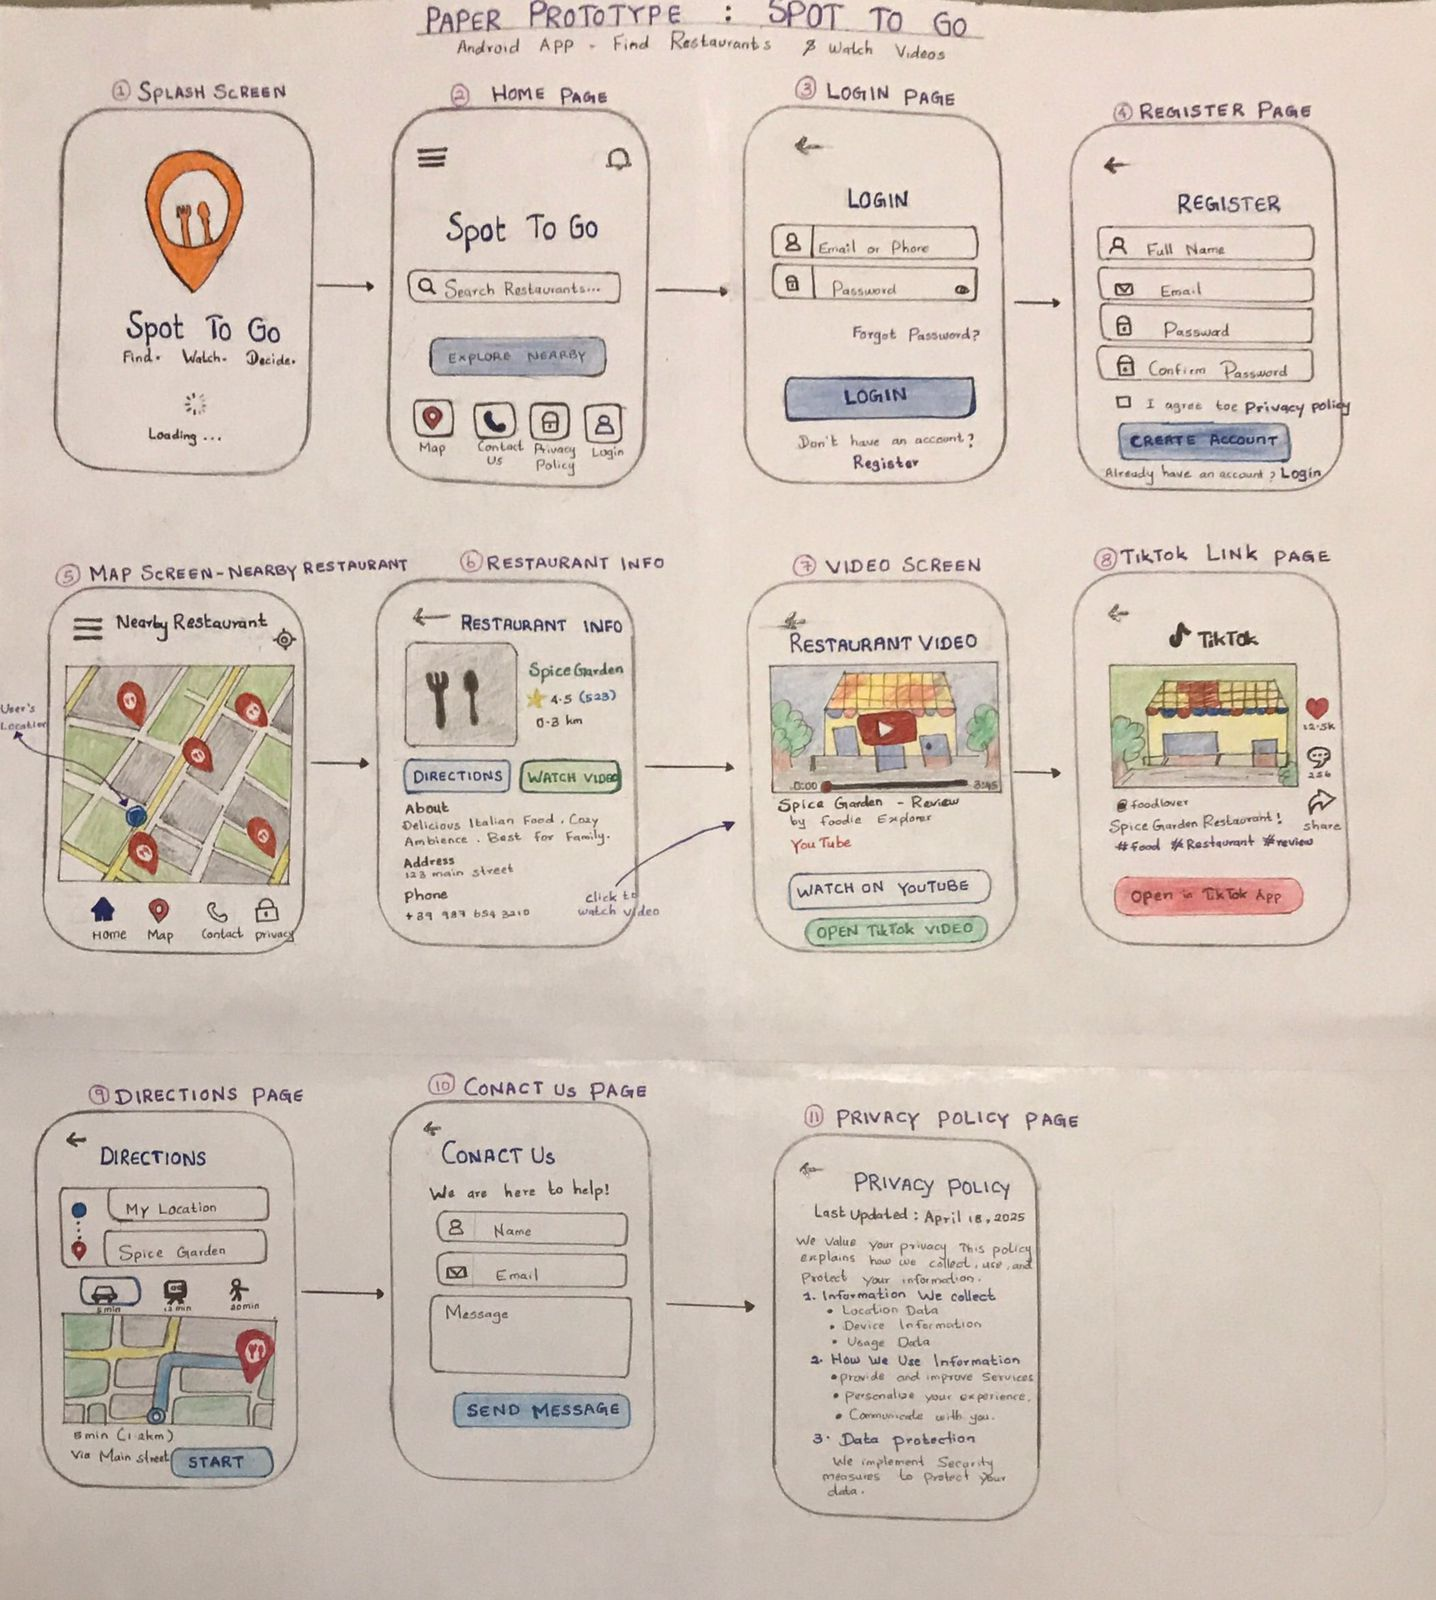
\includegraphics[width=0.92\textwidth]{prototype.jpeg}
    \caption{Prototype design of the Spot To Go application, illustrating the planned screen flow across six key views: the login screen, the home search interface, the interactive map with restaurant markers, the restaurant detail screen, the video playback screen, and the directions launcher. This layout directly informed the Activity-based architecture described above.}
    \label{fig:prototype}
\end{figure}

\subsection{Data Flow}

The following diagram illustrates the application's data flow. A location query from the user triggers a Places API request; the returned data populates the map as markers. Selecting a marker retrieves the associated video URL and routes to either the video platform or Google Maps navigation.

\begin{figure}[H]
\centering
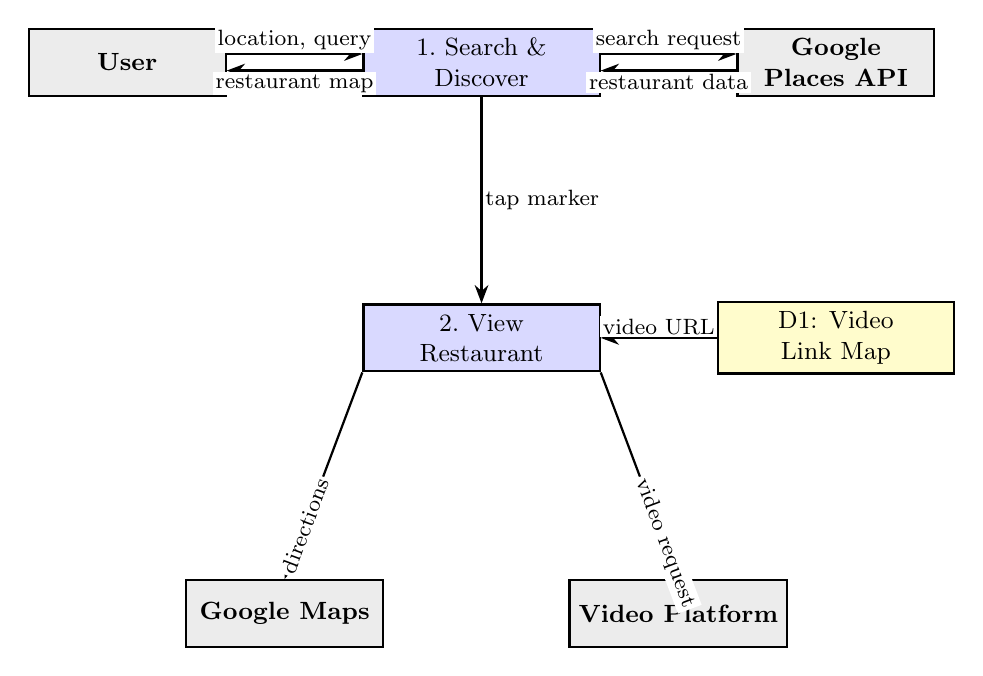
\begin{tikzpicture}[
    entity/.style={
        rectangle, draw, thick, fill=gray!15,
        minimum width=2.5cm, minimum height=0.85cm,
        align=center, font=\small\bfseries
    },
    process/.style={
        rectangle, draw, thick, fill=blue!15,
        minimum width=3cm, minimum height=0.85cm,
        align=center, font=\small
    },
    store/.style={
        rectangle, draw, thick, fill=yellow!20,
        minimum width=3cm, minimum height=0.85cm,
        align=center, font=\small
    },
    >=Stealth, thick,
    lbl/.style={font=\footnotesize, fill=white, inner sep=1pt}
]

\node[entity]  (user)   at (0,    0)    {User};
\node[process] (p1)     at (4.5,  0)    {1.\ Search \&\\Discover};
\node[entity]  (places) at (9,    0)    {Google\\Places API};
\node[process] (p2)     at (4.5, -3.5)  {2.\ View\\Restaurant};
\node[store]   (d1)     at (9,   -3.5)  {D1: Video\\Link Map};
\node[entity]  (maps)   at (2,   -7)    {Google Maps};
\node[entity]  (video)  at (7,   -7)    {Video Platform};

\draw[->] ([yshift= 3pt]user.east)    -- node[lbl, above]{location, query}   ([yshift= 3pt]p1.west);
\draw[->] ([yshift=-3pt]p1.west)      -- node[lbl, below]{restaurant map}    ([yshift=-3pt]user.east);
\draw[->] ([yshift= 3pt]p1.east)      -- node[lbl, above]{search request}    ([yshift= 3pt]places.west);
\draw[->] ([yshift=-3pt]places.west)  -- node[lbl, below]{restaurant data}   ([yshift=-3pt]p1.east);
\draw[->] (p1.south)                  -- node[lbl, right]{tap marker}        (p2.north);
\draw[->] (d1.west)                   -- node[lbl, above]{video URL}         (p2.east);
\draw[->] (p2.south west)             -- node[lbl, left,  sloped]{directions}    (maps.north);
\draw[->] (p2.south east)             -- node[lbl, right, sloped]{video request} (video.north);

\end{tikzpicture}
\caption{Level 1 Data Flow Diagram --- Spot To Go}
\label{fig:dfd}
\end{figure}

\subsection{Data Source and Restaurant Discovery}

Restaurant data is retrieved from the Google Places API using the Nearby Search endpoint. Each request is constructed with the user's current GPS coordinates, a search radius of 1,500 metres, and a type filter set to ``restaurant.'' The API response includes the restaurant name, address, star rating, and a stable \texttt{place\_id} identifier, which is used as the primary key throughout the application.

The user's location is obtained via the Android Fused Location Provider, which combines GPS, Wi-Fi, and mobile network signals for an accurate and battery-efficient estimate. Location permission is requested at runtime; if denied, the application degrades gracefully with an informative message.

\subsection{Video Integration}

Each restaurant is associated with a video URL (YouTube or TikTok) via a local data structure that maps \texttt{place\_id} values to video links. For the purpose of this project, a curated set of restaurants are pre-seeded with verified video URLs to demonstrate the feature. When a user selects the ``Watch Video'' option on the detail screen, the application either embeds the video using an Android \texttt{WebView} component or launches the platform's native application via an implicit Intent, depending on what is available on the device.

This approach avoids direct integration with restricted platforms while still demonstrating the full intended user experience within the academic scope.

\subsection{Evaluation}

The application is evaluated through structured functional testing against each of the seven defined objectives. For each objective, test cases are defined in advance covering expected behavior and edge cases such as permission denial, loss of connectivity, and missing video content. Results are documented against the success criteria, prioritizing verifiable, objective-by-objective assessment over automated test coverage.

\subsection{Usability Testing}

Functional testing verifies that features behave correctly; usability testing assesses whether the interface is intuitive for an unfamiliar user.

The first stage applies a heuristic inspection to each screen using Nielsen's ten usability heuristics \citep{nielsen1994}. This technique does not require participant recruitment and is well-suited to a single-developer academic project. The four heuristics most applicable here are visibility of system status, match between system and real world, user control and freedom, and error prevention. Identified issues are rated by severity, and any major or critical issues are resolved before final submission.

In the second stage, three to five participants complete a set of defined tasks — finding a restaurant, viewing its details, and accessing its video — without developer assistance. Task completion rate is recorded and participants complete a brief System Usability Scale (SUS) questionnaire. Findings from both stages are documented in the dissertation.

% ============================================================
\section{Analysis of Risks and Ethical Issues}

\subsection{Technical Risks}

The primary technical risk is dependency on the Google Places API, which operates under a daily request quota that could limit available calls during development and demonstration. This risk is managed by caching responses where stable and controlling request frequency during testing.

A secondary risk is the reliability of linked video content. Since URLs reference external platforms, a video may be removed or become unavailable without notice. This is mitigated by selecting stable videos for the demonstration and documenting this limitation within the application.

Device fragmentation is a further consideration, given Android's wide range of screen sizes, hardware configurations, and API levels. This risk is managed by testing on multiple emulator configurations and following Material Design guidelines, which scale predictably across screen sizes.

\subsection{Ethical Considerations}

The application accesses the user's GPS location solely for identifying nearby restaurants. This data is not stored beyond the active session and is only transmitted to the Google Places API as part of a standard API request. Location permission is requested explicitly; if denied, no location data is accessed.

The login and registration screens are included solely to demonstrate the system's authentication workflow and are not connected to a live authentication service. No real user credentials are collected, stored, or transmitted; access during demonstration is granted using hardcoded sample credentials. As a result, the application collects no personal data and presents no associated data security risk.

Given that this project does not involve the recruitment of human participants and collects no sensitive personal data, formal ethical approval is not required. The application is developed in accordance with the principles of data minimization and user transparency.

% ============================================================
\section{Project Work Plan and Gantt Chart}

The project is organized into seven work packages spanning seventeen weeks from April to August 2026, each corresponding to a phase of development.

\textbf{WP1 — Literature Review and Research (Weeks 1–3):} Review of related literature in location-based services, recommendation systems, and Android development. Identification of APIs, tools, and relevant technical constraints.

\textbf{WP2 — Environment Setup and Architecture Design (Weeks 2–4):} Configuration of Android Studio, integration of Google Play Services dependencies, and design of the Activity structure and data flow diagram.

\textbf{WP3 — Core Development: Maps and Location (Weeks 4–7):} Implementation of the Google Maps integration, Fused Location Provider configuration, and display of restaurant markers retrieved from the Places API.

\textbf{WP4 — Restaurant Detail and Video Integration (Weeks 7–10):} Development of the detail screen, video linking via WebView or Intent, and implementation of the directions feature.

\textbf{WP5 — Search and UI Refinement (Weeks 9–12):} Implementation of the keyword search bar, user interface refinements based on usability review, and layout testing across multiple screen configurations.

\textbf{WP6 — Testing and Dissertation Writing (Weeks 11–15):} Functional testing against all objectives, documentation of results, and completion of the dissertation report.

\textbf{WP7 — Presentation Preparation (Weeks 15–17):} Preparation and rehearsal of the final project presentation.

\vspace{1em}

% --- Gantt Chart ---
\begin{figure}[h!]
\centering
\begin{ganttchart}[
    hgrid,
    vgrid,
    x unit=0.67cm,
    y unit title=0.6cm,
    y unit chart=0.55cm,
    title height=1,
    bar height=0.6,
    bar/.style={fill=blue!40},
    title/.style={fill=gray!20},
    title label font=\small,
    bar label font=\small
]{1}{17}
    \gantttitle{Project Timeline (Weeks)}{17} \\
    \gantttitlelist{1,...,17}{1} \\
    \ganttbar{WP1: Literature Review}{1}{3} \\
    \ganttbar{WP2: Setup \& Architecture}{2}{4} \\
    \ganttbar{WP3: Maps \& Location}{4}{7} \\
    \ganttbar{WP4: Detail \& Video}{7}{10} \\
    \ganttbar{WP5: Search \& UI Polish}{9}{12} \\
    \ganttbar{WP6: Testing \& Writing}{11}{15} \\
    \ganttbar{WP7: Report \& Presentation}{15}{17}
\end{ganttchart}
\caption{Project Gantt Chart — Spot To Go (April–August 2026)}
\end{figure}

% ============================================================
\section{Conclusion}

This proposal has outlined the design and development plan for ``Spot To Go,'' an Android application that combines location-based restaurant discovery with video-based content integration. The application addresses a clear and practical gap in existing restaurant discovery tools: the absence of visual, experiential content at the point of decision-making.

The project is grounded in established research across four relevant areas — location-based services, recommendation systems, user-generated content, and Android development — and adopts a technically sound approach using well-documented tools. The defined objectives and Agile methodology together provide a structured and verifiable framework for development and evaluation.

Through this project, practical competency in Android development — including location services, REST API integration, and Activity-based architecture — will be developed and demonstrated. The result will be a functional, user-centered mobile application that meets the defined academic and technical requirements, and that lays a foundation for future enhancements such as personalized recommendations or natural language search.

% ============================================================
\newpage
\bibliographystyle{apalike}
\bibliography{references}

\end{document}
